\newif\ifsolutions
\solutionstrue % Show solutions
%\solutionsfalse % Hide solutions

\documentclass{article}
\usepackage{geometry}
\geometry{margin=1in}
\usepackage{tikz}
\usepackage{amssymb}

% fleqn allows setting indent of display math
\usepackage[fleqn]{amsmath}
\setlength{\mathindent}{0pt} % Set indent
% Disable equation numbering (https://tex.stackexchange.com/a/360378)
\makeatletter
\renewcommand\tagform@[1]{}
\makeatother

% Allow Unicode (some, e.g., © and £ at least)
% https://tex.stackexchange.com/questions/370278/is-there-any-reason-to-use-inputenc
\usepackage[utf8]{inputenc}

% Hyperlinks
\usepackage{hyperref}
\hypersetup{colorlinks=true, urlcolor=blue, linkcolor=blue}

% Prevent indentation of paragraphs
\setlength\parindent{0pt}
\setlength{\parskip}{\baselineskip}

% Spacing above/below equations
% https://tex.stackexchange.com/a/69678
\AtBeginDocument{%
 \abovedisplayskip=-\parskip
 \abovedisplayshortskip=-\parskip
 \belowdisplayskip=0pt
 \belowdisplayshortskip=0pt
}

% Allow 3 additional subsection levels
% https://tex.stackexchange.com/a/60212
\usepackage{titlesec}
\setcounter{secnumdepth}{6}
% H4 in HTML
\titleformat{\paragraph}{\normalfont\normalsize\bfseries}{\theparagraph}{1em}{}
\titlespacing*{\paragraph}{0pt}{3.25ex plus 1ex minus .2ex}{1.5ex plus .2ex}
% H5 in HTML
\titleformat{\subparagraph}{\normalfont\normalsize\bfseries}{\thesubparagraph}{1em}{}
\titlespacing*{\subparagraph}{0pt}{3.25ex plus 1ex minus .2ex}{1.5ex plus .2ex}
% H6 in HTML
\titleformat{\subsubparagraph}{\normalfont\normalsize\bfseries}{\thesubsubparagraph}{1em}{}
\titlespacing*{\subsubparagraph}{0pt}{3.25ex plus 1ex minus .2ex}{1.5ex plus .2ex}

% So enumerate at all levels is numbers
% https://tex.stackexchange.com/questions/78842/nested-enumeration-numbering
\renewcommand{\labelenumii}{\arabic{enumii}.}
\renewcommand{\labelenumiii}{\arabic{enumiii}.}
\renewcommand{\labelenumiv}{\arabic{enumiv}.}

\renewcommand{\mbox}{\text}
\newcommand{\ds}[0]{\displaystyle}
\newcommand{\ihat}[0]{\hat{\boldsymbol{\imath}}}
\newcommand{\jhat}[0]{\hat{\boldsymbol{\jmath}}}
\newcommand{\khat}[0]{\hat{\boldsymbol{k}}}
\newcommand{\xhat}[0]{\hat{\mathbf{x}}}
\newcommand{\yhat}[0]{\hat{\mathbf{y}}}
\newcommand{\zhat}[0]{\hat{\mathbf{z}}}
\newcommand{\rhat}[0]{\hat{\mathbf{r}}}
\newcommand{\bfvec}[1]{\vec{\mathbf{#1}}}
\newcommand{\bfcdot}[0]{\boldsymbol{\cdot}}

\usepackage{fancyhdr}
\pagestyle{fancy}
\lhead{Electric Force}
\rhead{\thepage}
\fancyfoot{}

\begin{document}

\section{Overview}

We generally describe vector equations in two ways:

\begin{enumerate}

  \item Simple -- An equation for the magnitude is given, and words are used to describe the direction.

  \item Compact -- A single equation is given for the vector, and additional equations are given for parts of the equation.

\end{enumerate}

For example, in Section 21.3 of the textbook, the equation for Coulomb's Law was given in the simple form. In Section 21.4, the equation for the electric field due to a point charge was given in the compact form.

In PHYS 260, you will need to be able to solve problems similar to the examples given here quickly. If you found the problems in this activity to be difficult, review Sections 1.7-1.8 in the textbook and see Khan Academy's comprehensive introduction to vectors.

\section{Coulomb's Law in Simple Form}

\emph{Magnitude}

\begin{equation}
F_{1\mbox{ on } 2}=k\frac{|q_1q_2|}{r^2}
\end{equation}

where $r$ is the distance between $q_1$ and $q_2$. To simplify notation, we are using $k$ in place of $1/4\pi\epsilon_o$.

\emph{Direction}

Along line that connects $q_1$ and $q_2$. Direction depends on signs of $q_1$ and $q_2$. (Likes repel, opposites attract.).

\subsection{Example}

Charge $q_1$ is at $(x,y)=(-a,-a)$ and charge $q_2$ is at $(a, a)$. Both charges have a charge of $q$.

\begin{enumerate}

  \item Find the magnitude and direction of the force of $q_1$ on $q_2$.

  \item Write the force of $q_1$ on $q_2$ in the form $\bfvec{F}=F_x\ihat + F_y\jhat$.

\end{enumerate}

\ifsolutions
\textbf{Solution}

    \begin{enumerate}

      \item The distance between the charges is $r=2\sqrt{2}a$, so

        \begin{equation}
        F_{1\mbox{ on } 2}=k\frac{|q_1q_2|}{r^2}=\frac{k|qq|}{(2\sqrt{2}a)^2}=\frac{kq^2}{8a^2}
        \end{equation}

            The charges will repel each other, so the direction of forces of one on the other will be as shown in the diagram. The direction of the force vector on $q_2$ is shown in the diagram.

            

\tikzset{every picture/.style={line width=0.75pt}} %set default line width to 0.75pt        

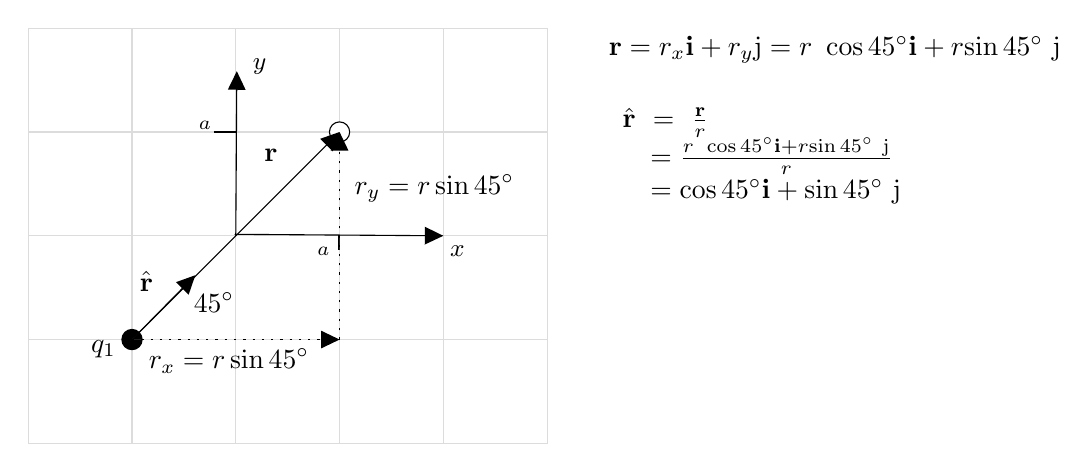
\begin{tikzpicture}[x=0.75pt,y=0.75pt,yscale=-1,xscale=1]
%uncomment if require: \path (0,227); %set diagram left start at 0, and has height of 227

%Shape: Grid [id:dp529276453314883] 
\draw  [draw opacity=0] (22.5,12) -- (272.5,12) -- (272.5,212) -- (22.5,212) -- cycle ; \draw  [color={rgb, 255:red, 220; green, 220; blue, 220 }  ,draw opacity=1 ] (72.5,12) -- (72.5,212)(122.5,12) -- (122.5,212)(172.5,12) -- (172.5,212)(222.5,12) -- (222.5,212) ; \draw  [color={rgb, 255:red, 220; green, 220; blue, 220 }  ,draw opacity=1 ] (22.5,62) -- (272.5,62)(22.5,112) -- (272.5,112)(22.5,162) -- (272.5,162) ; \draw  [color={rgb, 255:red, 220; green, 220; blue, 220 }  ,draw opacity=1 ] (22.5,12) -- (272.5,12) -- (272.5,212) -- (22.5,212) -- cycle ;
%Straight Lines [id:da9891788651841897] 
\draw    (122.5,112) -- (122.98,35.71) ;
\draw [shift={(123,32.71)}, rotate = 90.36] [fill={rgb, 255:red, 0; green, 0; blue, 0 }  ][line width=0.08]  [draw opacity=0] (8.93,-4.29) -- (0,0) -- (8.93,4.29) -- cycle    ;
%Straight Lines [id:da2531333242243323] 
\draw    (122,111.29) -- (219.5,111.98) ;
\draw [shift={(222.5,112)}, rotate = 180.41] [fill={rgb, 255:red, 0; green, 0; blue, 0 }  ][line width=0.08]  [draw opacity=0] (8.93,-4.29) -- (0,0) -- (8.93,4.29) -- cycle    ;
%Shape: Circle [id:dp928405560720714] 
\draw  [fill={rgb, 255:red, 0; green, 0; blue, 0 }  ,fill opacity=1 ] (67.63,162) .. controls (67.63,159.31) and (69.81,157.13) .. (72.5,157.13) .. controls (75.19,157.13) and (77.37,159.31) .. (77.37,162) .. controls (77.37,164.69) and (75.19,166.87) .. (72.5,166.87) .. controls (69.81,166.87) and (67.63,164.69) .. (67.63,162) -- cycle ;
%Shape: Circle [id:dp5390897406789283] 
\draw  [fill={rgb, 255:red, 255; green, 255; blue, 255 }  ,fill opacity=1 ] (167.63,62) .. controls (167.63,59.31) and (169.81,57.13) .. (172.5,57.13) .. controls (175.19,57.13) and (177.37,59.31) .. (177.37,62) .. controls (177.37,64.69) and (175.19,66.87) .. (172.5,66.87) .. controls (169.81,66.87) and (167.63,64.69) .. (167.63,62) -- cycle ;
%Straight Lines [id:da7315731890311423] 
\draw    (172.25,118.64) -- (172.25,111.64) ;
%Straight Lines [id:da41456511159458476] 
\draw    (112,62) -- (122.5,62) ;
%Straight Lines [id:da2368656312096422] 
\draw [fill={rgb, 255:red, 255; green, 255; blue, 255 }  ,fill opacity=1 ]   (72.5,162) -- (170.38,64.12) ;
\draw [shift={(172.5,62)}, rotate = 135] [fill={rgb, 255:red, 0; green, 0; blue, 0 }  ][line width=0.08]  [draw opacity=0] (8.93,-4.29) -- (0,0) -- (8.93,4.29) -- cycle    ;
%Straight Lines [id:da7182242007176092] 
\draw [fill={rgb, 255:red, 255; green, 255; blue, 255 }  ,fill opacity=1 ]   (72.5,162) -- (100.9,133.14) ;
\draw [shift={(103,131)}, rotate = 134.54] [fill={rgb, 255:red, 0; green, 0; blue, 0 }  ][line width=0.08]  [draw opacity=0] (8.93,-4.29) -- (0,0) -- (8.93,4.29) -- cycle    ;
%Straight Lines [id:da30412883702424365] 
\draw [fill={rgb, 255:red, 255; green, 255; blue, 255 }  ,fill opacity=1 ] [dash pattern={on 0.84pt off 2.51pt}]  (72.5,162) -- (169.5,162) ;
\draw [shift={(172.5,162)}, rotate = 180] [fill={rgb, 255:red, 0; green, 0; blue, 0 }  ][line width=0.08]  [draw opacity=0] (8.93,-4.29) -- (0,0) -- (8.93,4.29) -- cycle    ;
%Straight Lines [id:da8752471532648969] 
\draw [fill={rgb, 255:red, 255; green, 255; blue, 255 }  ,fill opacity=1 ] [dash pattern={on 0.84pt off 2.51pt}]  (172.5,162) -- (172.5,65) ;
\draw [shift={(172.5,62)}, rotate = 90] [fill={rgb, 255:red, 0; green, 0; blue, 0 }  ][line width=0.08]  [draw opacity=0] (8.93,-4.29) -- (0,0) -- (8.93,4.29) -- cycle    ;

% Text Node
\draw (129.5,25.4) node [anchor=north west][inner sep=0.75pt]  [font=\small]  {$y$};
% Text Node
\draw (224.5,115.4) node [anchor=north west][inner sep=0.75pt]  [font=\small]  {$x$};
% Text Node
\draw (160.5,116.4) node [anchor=north west][inner sep=0.75pt]  [font=\scriptsize]  {$a$};
% Text Node
\draw (103.5,55.4) node [anchor=north west][inner sep=0.75pt]  [font=\scriptsize]  {$a$};
% Text Node
\draw (135,69) node [anchor=north west][inner sep=0.75pt]   [align=left] {$\displaystyle \mathbf{r}$};
% Text Node
\draw (51.5,161) node [anchor=north west][inner sep=0.75pt]   [align=left] {$\displaystyle q_{1}$};
% Text Node
\draw (75,128) node [anchor=north west][inner sep=0.75pt]   [align=left] {$\displaystyle \hat{\mathbf{r}}$};
% Text Node
\draw (178.5,81) node [anchor=north west][inner sep=0.75pt]   [align=left] {$\displaystyle r_{y} =r\sin 45^{\circ }$};
% Text Node
\draw (79.37,165) node [anchor=north west][inner sep=0.75pt]   [align=left] {$\displaystyle r_{x} =r\sin 45^{\circ }$};
% Text Node
\draw (101,138) node [anchor=north west][inner sep=0.75pt]   [align=left] {$\displaystyle 45^{\circ }$};
% Text Node
\draw (301,47.4) node [anchor=north west][inner sep=0.75pt]    {$ \begin{array}{l}
\hat{\mathbf{r}} \ =\ \frac{\mathbf{r}}{r}\\
\ \ \ =\frac{r\ \cos 45\mathbf{^{\circ } i} +r\mathrm{\sin 45^{\circ } \ j}}{r}\\
\ \ \ =\cos 45\mathbf{^{\circ } i} +\mathrm{\sin 45^{\circ } \ j}
\end{array}$};
% Text Node
\draw (301,14.4) node [anchor=north west][inner sep=0.75pt]    {$\mathbf{r} =r_{x}\mathbf{i} +r_{y}\mathrm{j} =r\ \cos 45\mathbf{^{\circ } i} +r\mathrm{\sin 45^{\circ } \ j}$};


\end{tikzpicture}


      \item Let $F = F_{1\mbox{ on } 2}$ from part 1. to simplify notation. Then

            $\bfvec{F} = F\cos 45^\circ \ihat + F\sin 45^\circ \jhat$. Given that $\cos 45^\circ=\sin 45^\circ = \frac{1}{\sqrt{2}}$, we can also write

        \begin{equation}
        \bfvec{F} = F\left[\frac{1}{\sqrt{2}}\ihat + \frac{1}{\sqrt{2}}\jhat\right]
        \end{equation}

    \end{enumerate}
\fi

\subsection{Problem}

Charge $q_1$ is at $(x,y)=(a,a)$ and charge $q_2$ is at $(-a, -a)$. Both charges have a charge of $q$. Draw this charge configuration and then using the steps in the previous example,

\input{figures/grid-w100pct-w20pps-h200px-h20pps.tikz}

\begin{enumerate}

  \item Find the magnitude and direction of the force of $q_1$ on $q_2$.

  \item Write the force of $q_1$ on $q_2$ in the form $\bfvec{F}=F_x\ihat + F_y\jhat$.

\end{enumerate}

\section{Coulomb's Law in Compact Form}

\begin{equation}
\bfvec{F}_{1\mbox{ on } 2}=kq_1q_2\frac{\rhat}{r^2}
\end{equation}

$\bfvec{r}=\bfvec{r}_2-\bfvec{r}_1$ is the vector from the position of $q_1$ to the position of $q_2$, $\bfvec{r}_1$ is a vector from the origin to the location of $q_1$, and $\bfvec{r}_2$ is a vector from the origin to the location of $q_2$.

$r=|\bfvec{r}|=|\bfvec{r}_2-\bfvec{r}_1|$ is the distance from $q_1$ to $q_2$.

$\displaystyle\rhat=\frac{\bfvec{r}}{r}$ is the unit vector pointing from the position of $q_1$ to the position of $q_2$.

Although this form looks more complex, it requires basic steps to use.

\subsection{Example}

Charge $q_1$ is at $(x,y)=(-a,-a)$ and charge $q_2$ is at $(a, a)$. Both charges have a charge of $q$.

\begin{enumerate}

  \item Write the force of $q_1$ on $q_2$ in the form $\bfvec{F}=F_x\ihat + F_y\jhat$.

  \item Find the magnitude and direction of the force of $q_1$ on $q_2$.

\end{enumerate}

\ifsolutions
\textbf{Solution}

    \begin{enumerate}

      \item The vector from the origin to the location of $q_1$ is $\bfvec{r}_1=-a\ihat -a\jhat$

            The vector from the origin to the location of $q_2$ is $\bfvec{r}_2=a\ihat + a\jhat$

            The distance vector is $\bfvec{r}=\bfvec{r}_2-\bfvec{r}_1=2a\ihat+2a\jhat$

            The length of the distance vector is

            $r=|\bfvec{r}_2-\bfvec{r}_1|=\sqrt{(2a)^2 + (2a)^2} = 2\sqrt{2}a$

            The unit vector pointing from the position of $q_1$ to the position of $q_2$ is

        \begin{equation}
        \rhat=\frac{\bfvec{r}}{r}=\frac{1}{\sqrt{2}}\ihat + \frac{1}{\sqrt{2}}\jhat
        \end{equation}

            Inserting the above results into the equation

            $\displaystyle \bfvec{F}_{1\mbox{ on } 2}=kq_1q_2\frac{\rhat}{r^2}\quad$ gives

        \begin{equation}
        \bfvec{F}_{1\mbox{ on } 2}=
         kq^2\frac{\left[\frac{1}{\sqrt{2}}\ihat + \frac{1}{\sqrt{2}}\jhat\right]}{(2\sqrt{2}a)^2}
         \quad\text{ or }\quad
         \bfvec{F}_{1\mbox{ on } 2}=
         \frac{kq^2}{8a^2}\left[\frac{1}{\sqrt{2}}\ihat + \frac{1}{\sqrt{2}}\jhat\right]
         \end{equation}

            (Note that one can avoid the need to compute $\rhat$ by using the equivalent formula $\displaystyle \bfvec{F}_{1\mbox{ on } 2}=kq_1q_2{\bfvec{r}}/{r^3}$.)

      \item Let $\bfvec{F} = \bfvec{F}_{1\mbox{ on } 2}$ from part 1. to simplify notation. Then

        \begin{equation}
        F=|\bfvec{F}|=\frac{kq^2}{8a^2}\sqrt{\left(\frac{1}{\sqrt{2}}\right)^2 + \left(\frac{1}{\sqrt{2}}\right)^2}=\frac{kq^2}{8a^2}
        \end{equation}

            The angle is $\displaystyle \theta = \tan^{-1}\left(\frac{F_y}{F_x}\right) = \tan^{-1}\bigg( \frac{\frac{F}{\sqrt{2}}}{\frac{F}{\sqrt{2}}}\bigg)=45^\circ$

            See the margin note on page 16 of the textbook for an issue that may arise when using this formula to compute an angle.

    \end{enumerate}
\fi

\subsection{Problem}

Charge $q_1$ is at $(x,y)=(a,a)$ and charge $q_2$ is at $(-2a, -2a)$. Both charges have a charge of $q$. Using the steps in the previous example,

\begin{enumerate}

  \item Write the force of $q_1$ on $q_2$ in the form $\bfvec{F}=F_x\ihat + F_y\jhat$.

  \item Find the magnitude and direction of the force of $q_1$ on $q_2$.

\end{enumerate}

\end{document}